\chapter{Introduction}
\label{chap:intro}

\begin{flushright}
\begin{small}
\textit{Even in science, the object of research is no longer nature itself, but man's investigation of nature.}\\
Werner Heisenberg
\end{small}
\end{flushright}

\section{On the importance of glaciers}

Glaciers are fascinating natural systems to study. Their beauty is the consequence of complex interactions between climate and topography, creating  unique natural features that shape landscapes, ecosystems and even climates wherever they flow. These perennial ice masses originate in places allowing the accumulation of snow, that over the course of years gradually transform into firn and eventually ice. Due to gravity, this ice flows downwards, reaching lower elevations with higher temperatures where ice is lost through different processes of ablation, such as ice melting or calving \citep{ipcc_climate_2018}. The sum of all accumulation and ablation in a glacier determines its mass balance, which is essential to track the evolution of glaciers through time and their contribution to sea level rise (Fig. \ref{intro:fig1}). Glaciers are excellent climate proxies, adjusting their geometry and size to changes in climate. They represent a large part of the cryosphere, storing about 69\% of the world's fresh water. In their study, glaciers are often divided into mountain glaciers (Fig. \ref{intro:fig1}) and ice-sheets, which differ in size and geographical location, with ice-sheets being much larger than mountain glaciers and situated in Greenland and Antarctica \citep{benn_glaciers_2014}. 

Mountains are the water towers of the world, acting as buffers that store solid precipitation and distribute fresh water resources throughout the year \citep{immerzeel_importance_2020}. Glaciers play a major role in this, providing water resources during the warmest months well after all snow has melted. This late summer run-off is essential to many ecosystems and about 10\% of the global human population that live in mountain areas and the contiguous plains \citep{huss_global-scale_2018, cauvy-fraunie_global_2019,farinotti_large_2019}. Mountain areas are amongst the most affected regions by anthropogenic climate change, outpacing global warming  with an increase of 0.3ºC per decade \cite{ipcc_climate_2018}. These rapid changes in climate are causing a widespread retreat of glaciers (Fig. \ref{intro:fig1}), with many regions already having reached "peak water", i.e. the maximum in annual glacier run-off. Once this point is reached, glaciers progressively reduce their water contributions, altering the hydrological regime of watersheds \citep{huss_global-scale_2018}. The disappearance of glaciers produces an early release of accumulated precipitation in spring and early summer, with potential droughts in late summer \citep{brunner_future_2019}. These fast changes in mountain glaciers result in glaciers currently being important contributors to sea level rise (0.92 $\pm$ 0.39 mm a$^{-1}$), as much as the massive Antarctic and Greenland ice-sheets combined, despite representing less than 1\% of the ice on Earth \citep{zemp_global_2019, hock_glaciermip_2019}. 

\begin{figure*}[h]
\centering
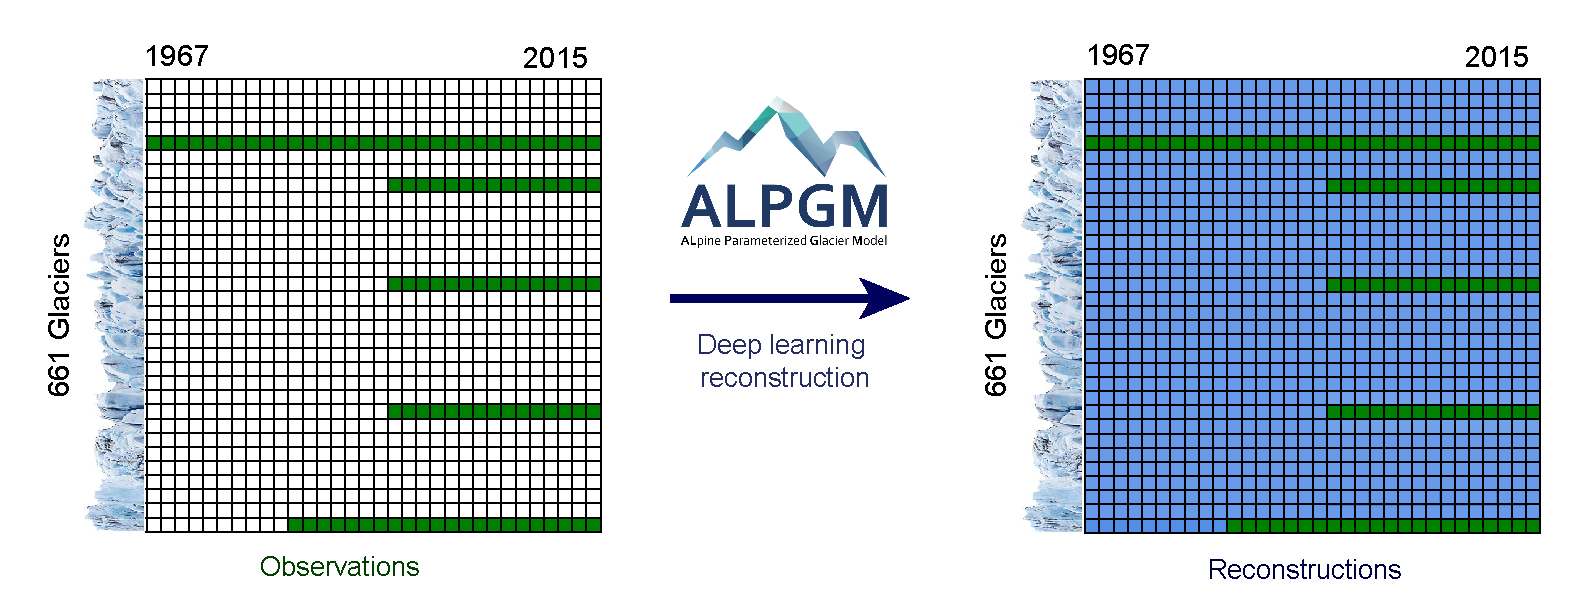
\includegraphics[width=14cm]{Figures/intro/Figure_1.png}
\caption{Glacier mass budgets for eleven different mountain regions and their combined results. Regional time series of annual mass change are based on glaciological and geodetic balances (Zemp et al., 2019). Superimposed are multi-year averages by Wouters et al. (2019) based on the Gravity Recovery and Climate Experiment (GRACE), only shown for the regions with glacier area >3,000 km2. Estimates by Gardner et al. (2013) were used in the IPCC 5th Assessment Report (AR5). Annual and time-averaged mass-budget estimates include the errors reported in each study. Glacier areas (A) and volumes (V) are based on RGI Consortium (2017)
and Farinotti et al. (2019), respectively. Red and blue bars on map refer to regional budgets averaged over the period 2006–2015 in units of kg m$^{–2}$ yr$^{–1}$ and mm sea level equivalent (SLE) yr$^{–1}$, respectively, and are derived from each region’s available mass-balance estimates. \textit{Figure from IPCC's Special Report on the Ocean and Cryosphere in a Changing Climate (SROCC, 2019).}} 
\label{intro:fig1}
\end{figure*}

Mountain glaciers are predicted to lose an important fraction of their overall mass by the end of the 21$^{st}$ century, with great differences between regions \citep{hock_glaciermip_2019}. The correct assessment of future glacier evolution is essential to understand and quantify the environmental and social consequences of their retreat. Since glaciers have become an icon of climate change, accurate predictions paired with effective communication can prove a great way to raise awareness on climate change. Despite scientific efforts to precisely quantify and understand glacier retreat, the main driver of future uncertainty in predictions are anthropogenic greenhouse emissions \citep{marzeion_partitioning_2020}. Scientific studies on glaciers must find their way into a wider audience in order to effectively contribute to their conservation. By combining an improved understanding of glacier processes with targeted communication of relevant results, we can aim at preserving our own very subject of study.  

\section{Glaciers in the French Alps}

\begin{wrapfigure}{R}{0.55\linewidth}
\centering
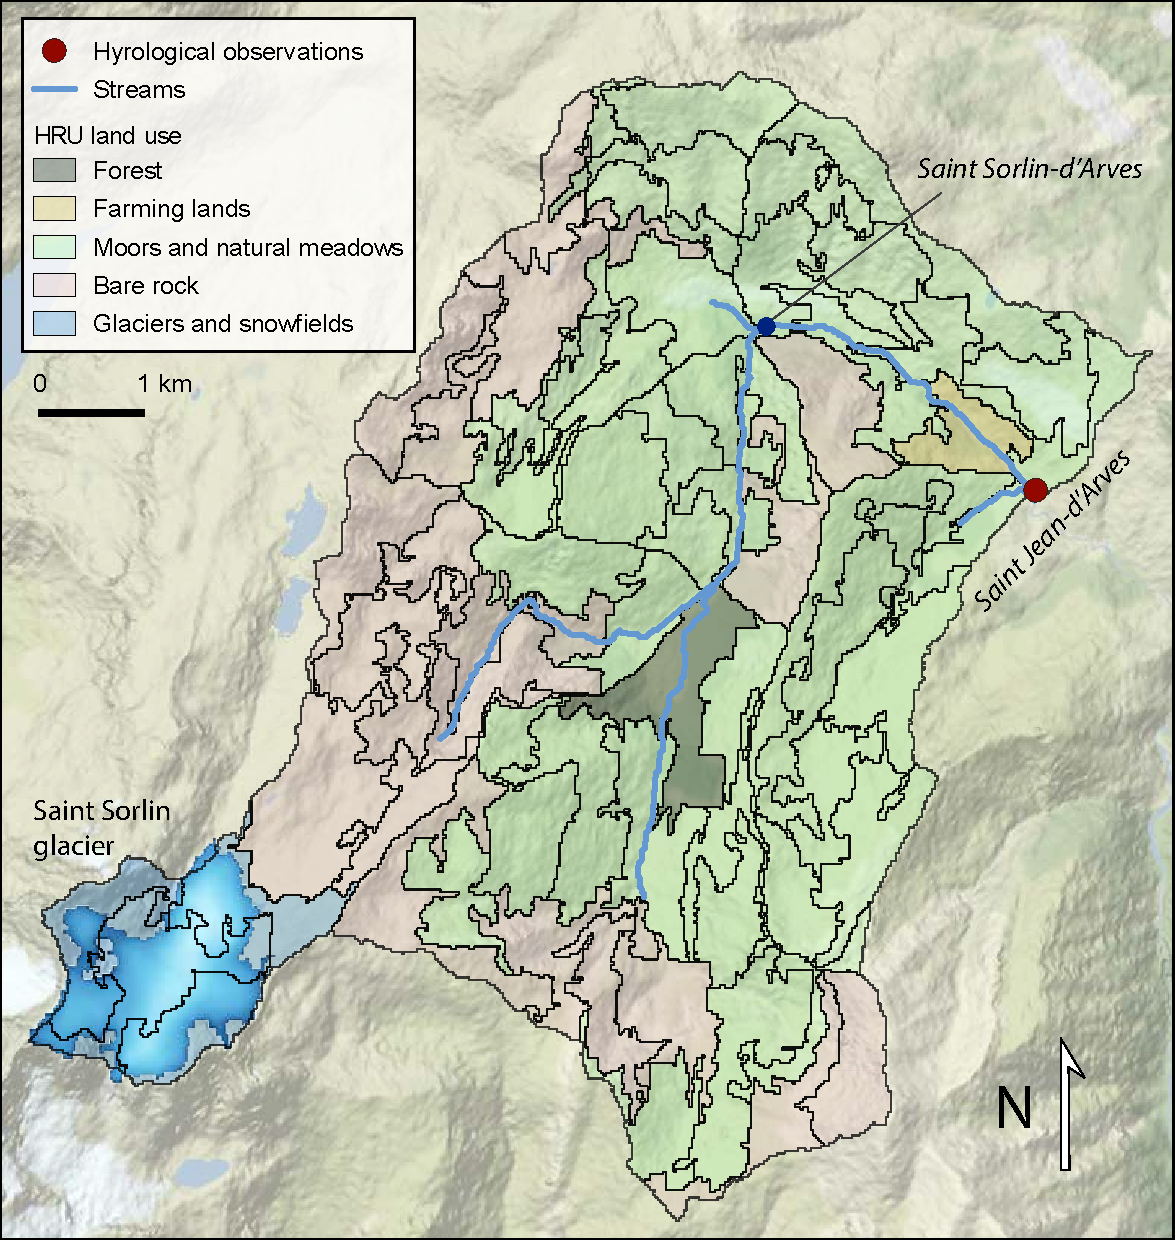
\includegraphics[width=8.3cm]{Figures/intro/Figure_2.pdf}
\caption{Glacierized massifs in the French Alps, with the extent of glaciers for the year 2015.}
\label{methods:fig4}
\end{wrapfigure}

The French Alps are located in the westernmost part of the European Alps, between 44º and 46º13'N and 5.08 and 7.67ºE. Their geographical location between the Mediterranean sea and continental Europe produces a particular climate gradient, from south-east to north-west. The southern massifs are more influenced by a Mediterranean climate, receiving less precipitation than their northern counterparts. Western Atlantic fluxes bring higher amounts of precipitation to north-western massifs, whereas eastern glaciers close to the Italian border receive most precipitation from east returns. These different climatic patterns, together with altitudes ranging from sea level to 4810 m at the summit of Mont Blanc, create an array of sub-climates that influence the evolution of glaciers. 

The French Alps have been inhabited for many centuries, developing a close relationship between alpine society and mountains. As for mountain peaks, the general social attitude towards glaciers has strongly evolved in the last centuries, transitioning from disdain and terror to awe and curiosity. This close relationship between society and glaciers has given them an important status in mountain culture, becoming symbols of identity for alpine societies throughout the European Alps. This means that the loss of glaciers has an additional consequence in the French Alps, on top of the environmental ones found in other glacierized regions. In many aspects, people in the French Alps have built their lives around mountains and glaciers, whose vast retreat will impact their socio-economic model. Emblematic regions such as the Mont-Blanc massif depend on glaciers for tourism, water resources and hydro-power generation. Moreover, natural hazards derived from glacier retreat might potentially impact populations in valleys. All these effects demand deep changes in the socio-economic model of these regions in order to correctly adapt to these changes in time. 

\section{Modelling large-scale glacier evolution}

\emph{"Enfin, combinant entre elles les trois causes qui contribuent à l'entretien des glaciers-réservoirs, il serait intéressant d'arriver à la masse qui leur est fournie chaque année ; mais on sent qu'il n'est possible d'avoir sur ce sujet que des conjectures plus ou moins vraisemblables ; c'est surtout ici que nous manquons et que nous manquerons toujours des observations qui doivent être le premier élément pour mener à l'intelligence de la nature."}

Predicting the future of glaciers is a complex task. It demands an understanding on the interplay of glacier processes that participate in glacier evolution. This is done by studying past glacier changes, in order to infer relationships between climate and topography, with the objective of acquiring equations and parametrizations of glacier processes. Nonetheless, future climate evolution depends on future greenhouse emissions, introducing large uncertainties in projections that cannot be avoided.  

\section{A short note to the reader}
\Blindtext